\section{Introduction}
% par 1: Introduction to the Problem
% Purpose: Define the problem and explain its significance.

%  What is the problem, what is the challenge, and why is it important
% Interfaces are important because they affect data collection. There is no QS interface, and QS is hard, so the problem is how do we design interfaces for QS?
Designing intuitive survey interfaces is crucial for accurately capturing respondents' preferences, which directly impact the quality and reliability of the data collected. For instance, voice assistants have been used to gather high-quality user feedback~\cite{xiaoLetMeAsk2021}, and a recent Human-Computer Interaction (HCI) study highlights that certain survey response formats can increase errors~\cite{pielotDidYouMisclick2024}. In this paper, our goal is to introduce an effective interface for~\textbf{Quadratic Surveys (QS)}, a survey tool designed to elicit preferences more accurately than traditional methods~\cite{chengCanShowWhat2021}. Despite the promise of QS, there has been no research on designing interfaces to support its unique quadratic mechanisms~\cite{grovesOptimalAllocationPublic1977}, where participants must rank and rate items --- a task that poses significant cognitive challenges. To popularize QS and ensure high-quality data, this paper addresses the question: \textit{How can we design interfaces to support participants in completing Quadratic Surveys (QS) more effectively?}

\begin{figure}[ht]
    \centering
    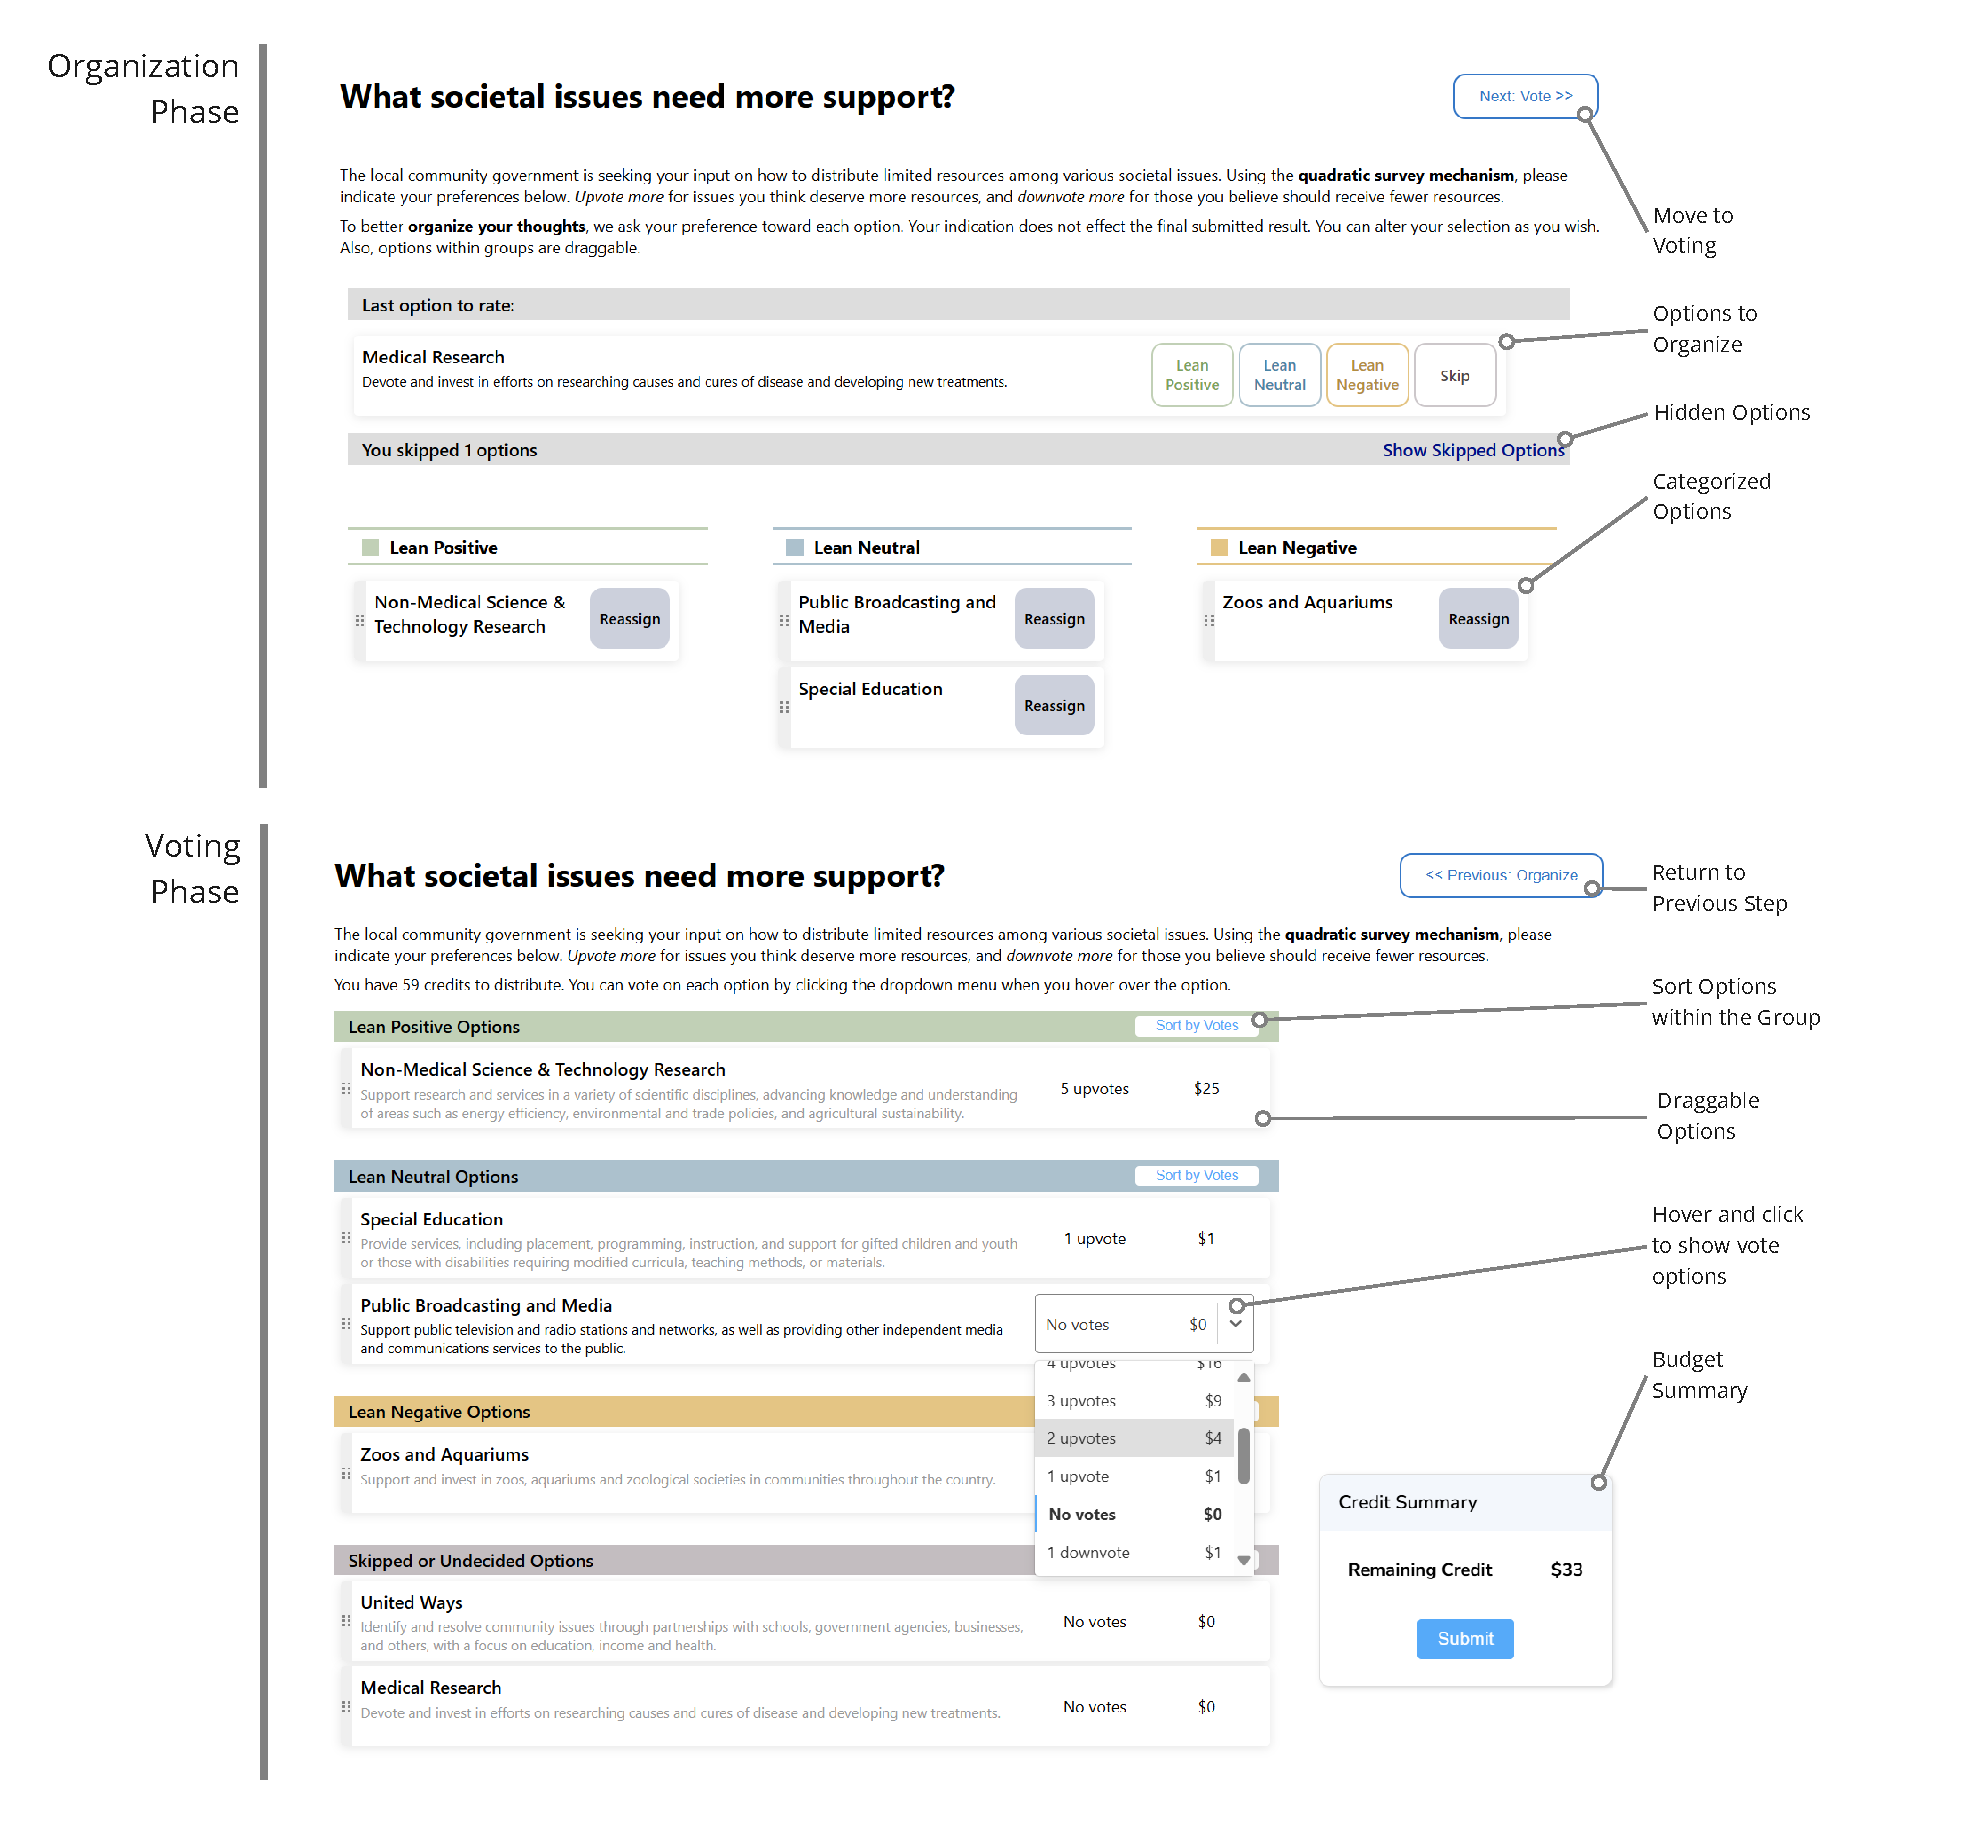
\includegraphics[width=1\textwidth]{content/image/detailed.pdf}
    \caption{The Two-Phase Interface: The interface consists of two phases. Survey respondents can navigate between phases using the top right button. In the organization phase, the interface presented one option at a time to the respondents where they choose among four choices: ``Lean Positive'', ``Lean Neutral'', ``Lean Negative'', or ``Skip''. Skipped options are hidden and can be evaluated later. The chosen options will be listed below. Items can be dragged and dropped across categories or returned to the stack. In the voting phase, options are listed in the order of the four categories. When hovering over each option, respondents can select a vote for that option using the dropdown. Each dropdown contains the cost associated with the vote. A sort button allows ascending sorting within each category. A summary box tracks the remaining credit balance.}
    \label{fig:interactiveInterface}
\end{figure}

% Zoom into two challenges this paper tackles -- zooming in mental demand and cognitive challenges due to the QS mechanism
We envision an effective interface that navigates participants through the complex mechanism and preference construction process, tailored to the unique challenges of QS. QS improves accuracy in individual preference elicitation compared to traditional methods like Likert scales by requiring participants to make trade-offs using a fixed budget of credits, where purchasing $k$ votes for an option in QS costs $k^2$ credits~\cite{quarfoot2017quadratic,chengCanShowWhat2021}. This quadratic cost structure forces respondents to carefully evaluate their preferences, balancing the strength of their support or opposition against the limited budget. While this cost structure forces them to make thoughtful trade-offs, this complexity also increases cognitive load, making it mentally taxing to weigh costs, evaluate options, and construct rankings~\cite{lichtensteinConstructionPreference2006}. Moreover, QS, often referred to as Quadratic Voting (QV) in voting scenarios, can involve hundreds of options~\cite{rogersColoradoTriedNew2019, teamTaiwanDigitalMinister}, increasing the risk of cognitive overload and satisficing~\cite{simonBehavioralModelRational1955, payneAdaptiveStrategySelection1988, tverskyJudgmentsRepresentativeness}. We propose that an effective interface tailored to support users through these complex trade-offs can reduce cognitive load and facilitate better preference construction.
% add and possible breakdown interfaces for mental and interfaces to scaffold complex mechanisms

% ================================ %
% par 2: Approaches to Address the Challenges
% Purpose: Describe the existing approaches related to the problem.
% Key Questions:
%  - What are some broad approaches to addressing these challenges? -- there are none.
%  - Do not go into detail about related work but give an idea of the major themes in related work.
%       - No prior research on QS, but there are existing interfaces -> auto calculation as commonality
%       - prior work on interface for reducing cognitive load, preference construction, and voting

To date, existing quadratic mechanism-powered applications simply present options, allow vote adjustments and automatically calculate votes, costs, and budget usage. These designs focused heavily on the mechanism, rather than supporting possible challenges these application users faced. Survey interface literature, while addressing decision-making and usability, most focus on traditional surveys that do not share the unique option-to-option trade-offs that QS introduces~\cite{engstrom2020politics, weijtersEffectRatingScale2010, kierujVariationsResponseStyle2010, toepoelSmileysStarsHearts2019, farzandAestheticsEvaluatingResponse2024, pielotDidYouMisclick2024}. The challenges, in particular, cognitive load~\cite{paula2023, norman2013design, toepoelSmileysStarsHearts2019, softwareBrad2021} and scaffolding challenging tasks~\cite{task2014, moderate2021, amyChatSensing2018} like preference construction, are opportunities where user interfaces have shown their promises. As a result, it remains unclear how different interface designs might support QS in reducing cognitive load and aiding preference construction.

% ================================ %
% par 3: Your Proposal
% Purpose: Present your main ideas and proposed solution.
% Key Question:
%  - What are you proposing? Provide a sketch of the major ideas.

After multiple design iterations, we propose a novel interactive two-phase ``organize-then-vote'' QS interface (two-phase interface, Figure~\ref{fig:interactiveInterface}) that integrates three key elements. First, the interface scaffolds the preference construction process by having participants initially categorize the survey options into ``Lean Positive,'' ``Lean Neutral,'' or ``Lean Negative.'' This serves as a cognitive warm-up, easing participants into the more complex QS voting task. Second, the interface arranges the options according to these categorizations, providing a structured visual layout. Third, participants can refine the positions of these options using drag-and-drop functionality, giving them greater control and agency in the preference-construction process. These design features are aligned with preference construction theory and build upon prior research in interface design to reduce cognitive load and enhance user engagement.

To explore how these interface elements mitigate the cognitive load and support preference construction in Quadratic Surveys, we pose the following research questions:
\begin{itemize}
    \item RQ1. How does the number of options in Quadratic Surveys impact respondents' cognitive load?
    \item RQ2a. How does the two-phase interface impact respondents' cognitive load compared to a text interface?
    \item RQ2b. What are the similarities and differences in sources of cognitive load across the two interfaces?
    \item RQ3. What are the differences in Quadratic Survey respondents' behaviors when coping with long lists of options across the two-phase interface and the text interface?
\end{itemize}

% ================================ %
% par 4: Main Findings
% Purpose: Summarize the key findings from your work.
% Key Question:
%  - What are the main findings?
We invited 41 participants to a lab study comparing our two-phase interface with a baseline to understand how different interface designs and option lengths ($6$ options or $24$ options) impact cognitive load. Qualitative findings, measured using the NASA Task Load Index~(NASA-TLX) and semi-structured interviews, revealed that participants using the two-phase interface experienced cognitive demand more from strategic, holistic thinking compared to personal relevance and operational tasks, particularly in longer surveys. Quantitative results showed that, although participants spent more time per option, they made faster decisions during the voting phase, suggesting a more efficient distribution of cognitive effort. We concluded that the two-phase interface prevented cognitive overload in long QS surveys and shifted mental load toward more strategic thinking, reducing reliance on mental shortcuts like satisficing~\cite{simonBehavioralModelRational1955}.

% ================================ %
% par 5: Main Contributions
% Purpose: Identify and explain the primary contributions of your work.
% Key Structure:
%  1. Line 1: Identify your contribution—conceptualization, framework, interface, algorithm, etc.
%  2. Line 2: Contrast your contribution with prior work.
%  3. Line 3: Explain how you accomplished your contribution.
%  4. Line 4: Emphasize the impact of the contribution—why should anyone care?

\paragraph{Contributions}
We contribute to the HCI community by proposing the first interface specifically designed for QS and QV-like applications, aimed at reducing cognitive challenges and scaffolding preference construction through a two-phase interface with direct manipulation. Before our work, no research had explored QS interfaces, particularly for long surveys prone to cognitive overload. Few studies in HCI address interfaces for surveys and questionnaires. Our study demonstrated how user interfaces can facilitate preference construction in situ and reduce satisficing behaviors by promoting incremental updates and deeper engagement with survey items through interface elements. Additionally, our interview is also the first in-depth qualitative analysis of user experiences with Quadratic Mechanism applications, identifying key factors contributing to cognitive load. The impact of our contribution extends beyond QS, offering design implications for other preference-elicitation tools in complex scenarios. By making QS easier to use and more accurate, our design also encourages wider adoption among researchers and practitioners. Finally, our work lays the groundwork for future studies on qualitative insights and future interface designs of quadratic mechanisms, supporting decision-makers in eliciting accurate respondents' preferences.

% ================================ %
% Removed text
% Surveys are a ubiquitous tool for collective decision-making, providing decision-makers with aggregated opinions that directly shape the outcomes for those surveyed. For example, states utilize referendums to form policy decisions, organizations like the Pew Research Center survey public perspectives on societal challenges in the United States, and city councils hold forums to gather community concerns.
% and private sectors~\cite{Gov4gitDecentralizedPlatform2023}.
% xiaoTellMeYourself2020, 

% ================================ %